%\renewcommand{\thefigure}{\theenumi}
%\renewcommand{\thetable}{\theenumi}
\renewcommand{\theequation}{\theenumi}
\begin{enumerate}[label=\thesection.\arabic*.,ref=\thesection.\theenumi]
\numberwithin{equation}{enumi}
\numberwithin{table}{enumi}


\item Two dice, one blue and one grey, are thrown at the same time.  
\begin{enumerate}
\item  Complete Table \ref{table:1.2.133}.
\item  A student argues that there are 11 possible outcomes 2, 3, 4, 5, 6, 7, 8, 9, 10, 11 and 12. Therefore, each of them has a probability $\frac{1}{11}$. Do you agree with this argument? Justify your answer.
\end{enumerate}
%
\begin{table}[ht!]
\centering
%%%%%%%%%%%%%%%%%%%%%%%%%%%%%%%%%%%%%%%%%%%%%%%%%%%%%%%%%%%%%%%%%%%%%%
%%                                                                  %%
%%  This is the header of a LaTeX2e file exported from Gnumeric.    %%
%%                                                                  %%
%%  This file can be compiled as it stands or included in another   %%
%%  LaTeX document. The table is based on the longtable package so  %%
%%  the longtable options (headers, footers...) can be set in the   %%
%%  preamble section below (see PRAMBLE).                           %%
%%                                                                  %%
%%  To include the file in another, the following two lines must be %%
%%  in the including file:                                          %%
%%        \def\inputGnumericTable{}                                 %%
%%  at the beginning of the file and:                               %%
%%        \input{name-of-this-file.tex}                             %%
%%  where the table is to be placed. Note also that the including   %%
%%  file must use the following packages for the table to be        %%
%%  rendered correctly:                                             %%
%%    \usepackage[latin1]{inputenc}                                 %%
%%    \usepackage{color}                                            %%
%%    \usepackage{array}                                            %%
%%    \usepackage{longtable}                                        %%
%%    \usepackage{calc}                                             %%
%%    \usepackage{multirow}                                         %%
%%    \usepackage{hhline}                                           %%
%%    \usepackage{ifthen}                                           %%
%%  optionally (for landscape tables embedded in another document): %%
%%    \usepackage{lscape}                                           %%
%%                                                                  %%
%%%%%%%%%%%%%%%%%%%%%%%%%%%%%%%%%%%%%%%%%%%%%%%%%%%%%%%%%%%%%%%%%%%%%%



%%  This section checks if we are begin input into another file or  %%
%%  the file will be compiled alone. First use a macro taken from   %%
%%  the TeXbook ex 7.7 (suggestion of Han-Wen Nienhuys).            %%
\def\ifundefined#1{\expandafter\ifx\csname#1\endcsname\relax}


%%  Check for the \def token for inputed files. If it is not        %%
%%  defined, the file will be processed as a standalone and the     %%
%%  preamble will be used.                                          %%
\ifundefined{inputGnumericTable}

%%  We must be able to close or not the document at the end.        %%
	\def\gnumericTableEnd{\end{document}}


%%%%%%%%%%%%%%%%%%%%%%%%%%%%%%%%%%%%%%%%%%%%%%%%%%%%%%%%%%%%%%%%%%%%%%
%%                                                                  %%
%%  This is the PREAMBLE. Change these values to get the right      %%
%%  paper size and other niceties.                                  %%
%%                                                                  %%
%%%%%%%%%%%%%%%%%%%%%%%%%%%%%%%%%%%%%%%%%%%%%%%%%%%%%%%%%%%%%%%%%%%%%%

	\documentclass[12pt%
			  %,landscape%
                    ]{report}
       \usepackage[latin1]{inputenc}
       \usepackage{fullpage}
       \usepackage{color}
       \usepackage{array}
       \usepackage{longtable}
       \usepackage{calc}
       \usepackage{multirow}
       \usepackage{hhline}
       \usepackage{ifthen}

	\begin{document}


%%  End of the preamble for the standalone. The next section is for %%
%%  documents which are included into other LaTeX2e files.          %%
\else

%%  We are not a stand alone document. For a regular table, we will %%
%%  have no preamble and only define the closing to mean nothing.   %%
    \def\gnumericTableEnd{}

%%  If we want landscape mode in an embedded document, comment out  %%
%%  the line above and uncomment the two below. The table will      %%
%%  begin on a new page and run in landscape mode.                  %%
%       \def\gnumericTableEnd{\end{landscape}}
%       \begin{landscape}


%%  End of the else clause for this file being \input.              %%
\fi

%%%%%%%%%%%%%%%%%%%%%%%%%%%%%%%%%%%%%%%%%%%%%%%%%%%%%%%%%%%%%%%%%%%%%%
%%                                                                  %%
%%  The rest is the gnumeric table, except for the closing          %%
%%  statement. Changes below will alter the table's appearance.     %%
%%                                                                  %%
%%%%%%%%%%%%%%%%%%%%%%%%%%%%%%%%%%%%%%%%%%%%%%%%%%%%%%%%%%%%%%%%%%%%%%

\providecommand{\gnumericmathit}[1]{#1} 
%%  Uncomment the next line if you would like your numbers to be in %%
%%  italics if they are italizised in the gnumeric table.           %%
%\renewcommand{\gnumericmathit}[1]{\mathit{#1}}
\providecommand{\gnumericPB}[1]%
{\let\gnumericTemp=\\#1\let\\=\gnumericTemp\hspace{0pt}}
 \ifundefined{gnumericTableWidthDefined}
        \newlength{\gnumericTableWidth}
        \newlength{\gnumericTableWidthComplete}
        \newlength{\gnumericMultiRowLength}
        \global\def\gnumericTableWidthDefined{}
 \fi
%% The following setting protects this code from babel shorthands.  %%
 \ifthenelse{\isundefined{\languageshorthands}}{}{\languageshorthands{english}}
%%  The default table format retains the relative column widths of  %%
%%  gnumeric. They can easily be changed to c, r or l. In that case %%
%%  you may want to comment out the next line and uncomment the one %%
%%  thereafter                                                      %%
\providecommand\gnumbox{\makebox[0pt]}
%%\providecommand\gnumbox[1][]{\makebox}

%% to adjust positions in multirow situations                       %%
\setlength{\bigstrutjot}{\jot}
\setlength{\extrarowheight}{\doublerulesep}

%%  The \setlongtables command keeps column widths the same across  %%
%%  pages. Simply comment out next line for varying column widths.  %%
\setlongtables

\setlength\gnumericTableWidth{%
	53pt+%
	53pt+%
0pt}
\def\gumericNumCols{2}
\setlength\gnumericTableWidthComplete{\gnumericTableWidth+%
         \tabcolsep*\gumericNumCols*2+\arrayrulewidth*\gumericNumCols}
\ifthenelse{\lengthtest{\gnumericTableWidthComplete > \linewidth}}%
         {\def\gnumericScale{\ratio{\linewidth-%
                        \tabcolsep*\gumericNumCols*2-%
                        \arrayrulewidth*\gumericNumCols}%
{\gnumericTableWidth}}}%
{\def\gnumericScale{1}}

%%%%%%%%%%%%%%%%%%%%%%%%%%%%%%%%%%%%%%%%%%%%%%%%%%%%%%%%%%%%%%%%%%%%%%
%%                                                                  %%
%% The following are the widths of the various columns. We are      %%
%% defining them here because then they are easier to change.       %%
%% Depending on the cell formats we may use them more than once.    %%
%%                                                                  %%
%%%%%%%%%%%%%%%%%%%%%%%%%%%%%%%%%%%%%%%%%%%%%%%%%%%%%%%%%%%%%%%%%%%%%%

\ifthenelse{\isundefined{\gnumericColA}}{\newlength{\gnumericColA}}{}\settowidth{\gnumericColA}{\begin{tabular}{@{}p{53pt*\gnumericScale}@{}}x\end{tabular}}
\ifthenelse{\isundefined{\gnumericColB}}{\newlength{\gnumericColB}}{}\settowidth{\gnumericColB}{\begin{tabular}{@{}p{53pt*\gnumericScale}@{}}x\end{tabular}}

\begin{tabular}[c]{%
	b{\gnumericColA}%
	b{\gnumericColB}%
	}

%%%%%%%%%%%%%%%%%%%%%%%%%%%%%%%%%%%%%%%%%%%%%%%%%%%%%%%%%%%%%%%%%%%%%%
%%  The longtable options. (Caption, headers... see Goosens, p.124) %%
%	\caption{The Table Caption.}             \\	%
% \hline	% Across the top of the table.
%%  The rest of these options are table rows which are placed on    %%
%%  the first, last or every page. Use \multicolumn if you want.    %%

%%  Header for the first page.                                      %%
%	\multicolumn{2}{c}{The First Header} \\ \hline 
%	\multicolumn{1}{c}{colTag}	%Column 1
%	&\multicolumn{1}{c}{colTag}	\\ \hline %Last column
%	\endfirsthead

%%  The running header definition.                                  %%
%	\hline
%	\multicolumn{2}{l}{\ldots\small\slshape continued} \\ \hline
%	\multicolumn{1}{c}{colTag}	%Column 1
%	&\multicolumn{1}{c}{colTag}	\\ \hline %Last column
%	\endhead

%%  The running footer definition.                                  %%
%	\hline
%	\multicolumn{2}{r}{\small\slshape continued\ldots} \\
%	\endfoot

%%  The ending footer definition.                                   %%
%	\multicolumn{2}{c}{That's all folks} \\ \hline 
%	\endlastfoot
%%%%%%%%%%%%%%%%%%%%%%%%%%%%%%%%%%%%%%%%%%%%%%%%%%%%%%%%%%%%%%%%%%%%%%

\hhline{|-|-}
	 \multicolumn{1}{|p{\gnumericColA}|}%
	{\gnumericPB{\raggedright}\gnumbox[l]{\textbf{Event}}}
	&\multicolumn{1}{p{\gnumericColB}|}%
	{\gnumericPB{\raggedright}\gnumbox[l]{\textbf{Value}}}
\\
\hhline{|--|}
	 \multicolumn{1}{|p{\gnumericColA}|}%
	{\gnumericPB{\raggedleft}\gnumbox[r]{2}}
	&\multicolumn{1}{p{\gnumericColB}|}%
	{\gnumericPB{\raggedright}\gnumbox[l]{1/36}}
\\
\hhline{|--|}
	 \multicolumn{1}{|p{\gnumericColA}|}%
	{\gnumericPB{\raggedleft}\gnumbox[r]{3}}
	&\multicolumn{1}{p{\gnumericColB}|}%
	{\gnumericPB{\raggedright}\gnumbox[l]{-}}
\\
\hhline{|--|}
	 \multicolumn{1}{|p{\gnumericColA}|}%
	{\gnumericPB{\raggedleft}\gnumbox[r]{4}}
	&\multicolumn{1}{p{\gnumericColB}|}%
	{\gnumericPB{\raggedright}\gnumbox[l]{-}}
\\
\hhline{|--|}
	 \multicolumn{1}{|p{\gnumericColA}|}%
	{\gnumericPB{\raggedleft}\gnumbox[r]{5}}
	&\multicolumn{1}{p{\gnumericColB}|}%
	{\gnumericPB{\raggedright}\gnumbox[l]{-}}
\\
\hhline{|--|}
	 \multicolumn{1}{|p{\gnumericColA}|}%
	{\gnumericPB{\raggedleft}\gnumbox[r]{6}}
	&\multicolumn{1}{p{\gnumericColB}|}%
	{\gnumericPB{\raggedright}\gnumbox[l]{-}}
\\
\hhline{|--|}
	 \multicolumn{1}{|p{\gnumericColA}|}%
	{\gnumericPB{\raggedleft}\gnumbox[r]{7}}
	&\multicolumn{1}{p{\gnumericColB}|}%
	{\gnumericPB{\raggedright}\gnumbox[l]{-}}
\\
\hhline{|--|}
	 \multicolumn{1}{|p{\gnumericColA}|}%
	{\gnumericPB{\raggedleft}\gnumbox[r]{8}}
	&\multicolumn{1}{p{\gnumericColB}|}%
	{\gnumericPB{\raggedright}\gnumbox[l]{5/36}}
\\
\hhline{|--|}
	 \multicolumn{1}{|p{\gnumericColA}|}%
	{\gnumericPB{\raggedleft}\gnumbox[r]{9}}
	&\multicolumn{1}{p{\gnumericColB}|}%
	{\gnumericPB{\raggedright}\gnumbox[l]{-}}
\\
\hhline{|--|}
	 \multicolumn{1}{|p{\gnumericColA}|}%
	{\gnumericPB{\raggedleft}\gnumbox[r]{10}}
	&\multicolumn{1}{p{\gnumericColB}|}%
	{\gnumericPB{\raggedright}\gnumbox[l]{-}}
\\
\hhline{|--|}
	 \multicolumn{1}{|p{\gnumericColA}|}%
	{\gnumericPB{\raggedleft}\gnumbox[r]{11}}
	&\multicolumn{1}{p{\gnumericColB}|}%
	{\gnumericPB{\raggedright}\gnumbox[l]{-}}
\\
\hhline{|--|}
	 \multicolumn{1}{|p{\gnumericColA}|}%
	{\gnumericPB{\raggedleft}\gnumbox[r]{12}}
	&\multicolumn{1}{p{\gnumericColB}|}%
	{\gnumericPB{\raggedright}\gnumbox[l]{1/36}}
\\
\hhline{|-|-|}
\end{tabular}

\ifthenelse{\isundefined{\languageshorthands}}{}{\languageshorthands{\languagename}}
\gnumericTableEnd

\caption{Input Values}
\label{table:1.2.133}	
\end{table}
\item A die is thrown once. Find the probability of getting\\
(i) a prime number;\\
(ii) a number lying between 2 and 6;\\
(iii) an odd number.
\\
\solution
Let X be the random variable representing the number of defective eggs from the ten eggs picked. X follows a  binomial distribution.  Since the probability of an egg being defective is 10\%, substituting n=10, p= 0.1 and k=0 in equation \eqref{eq:exam41_1}, 
probability that there is atleast one defective egg is 
\begin{align}
\pr{X \geq 1}&= 1 - \pr{X=0}  = 1-\brak{0.9}^{10}
\\
&=0.6513215599
\end{align}
The python code for the above problem is,
\begin{lstlisting}
.solutions/20-10/prob/codes/exam42.py
\end{lstlisting}

\item In a game, a man wins a rupee for a six and loses a rupee for any other number when a fair die is thrown. The man decided to throw a die thrice but to quit as and when he gets a six. Find the expected value of the amount he wins / loses.\\
\item 
\item Find the probability of getting 5 exactly twice in 7 throws of a die.\\
\solution
There are 6 outcomes when we throw a die, which are independent of one another. The probability of getting 5 on the die 
\begin{align}
    p = \frac{1}{6}
\end{align}
The die is thrown 7 times and are not dependent on one another \begin{align}
    n = 7
\end{align}
Let the Random Variable be $X$ denote the number of 5s in 7 throws
By Binomial Distribution, we have
\begin{align}
    \Pr(X=k) = \binom{n}{k}p^k(1-p)^{n-k}
\end{align}
We should get 5 exactly twice, so $ k = 2 $\\
\begin{center}
\begin{table}[h]
\caption{Definition of the variables}
\centering
\resizebox{\columnwidth}{!}{%
    \begin{tabular}{|c|c|}
        \hline
         \multicolumn{2}{|c|}{Variables} \\
        \hline
        $p$ & Probability that outcome is 5 when we throw the die\\
        \hline
        $n$ & No of times the die is thrown\\
        \hline
        $X$ & Random Variable denoting the number of 5s out of n number of throws\\
        \hline
        $k$ & Required number of times 5s appear on the die which is 2\\
        \hline
    \end{tabular}
    }
    \label{tab:1}
\end{table}
\end{center}
The probability of getting 5 exactly twice in 7 throws of a die is given by 
\begin{align}
    \Pr(X=2) &= \comb{^7}{C}{_2}\brak{\frac{1}{6}}^2 \brak{\frac{5}{6}}^5 \\[7pt]
    \Pr(X=2) &= 0.234428
\end{align}


\item 

\item
\item 
\item Let X denote the sum of the numbers obtained when two fair dice are rolled. Find the variance and standard deviation of X.\\
\solution
When two fare dice are rolled. The sum of the numbers obtained can have the values 2, 3, 4, 5, 6, 7, 8, 9, 10, 11, 12.\\
$\pr{X}$ = probability of obtaining X as the sum and let us represent the case when first dice shows the number $x_1$ and the second dice shows the number $x_2$ as $(x_1,x_2)$.
\begin{table}[hbt!]
\resizebox{\columnwidth}{!}{
\begin{tabular}{|l|c|c|c|c|c|c|c|c|c|c|c|}
\hline
\multicolumn{1}{|c|}{x} & 2 & 3 & 4 & 5 & 6 & 7 & 8 & 9 & 10 & 11 & 12 \\ \hline
$\pr{X}$                   &$\frac{1}{36}$   &$\frac{2}{36}$   &$\frac{3}{36}$   &$\frac{4}{36}$   &$\frac{5}{36}$   &$\frac{6}{36}$   &$\frac{5}{36}$   &$\frac{4}{36}$   &$\frac{3}{36}$    &$\frac{2}{36}$    &$\frac{1}{36}$    \\ \hline
\end{tabular}
}
\caption{Probability Distribution Table of X}
\label{table:1}
\end{table}
For the above problem,we know that.
\begin{align}
p_x\brak{n} &= 
  \begin{cases}
    0 & \text{if } n \leq 1,\\
    \frac{n-1}{36} & \text{if } 2 \leq n \leq 7,\\
    \frac{13-n}{36} & \text{if } 7 < n \leq 12,\\
    0 & \text{if } n>12.
  \end{cases}
\end{align}
\begin{align}
    &Mean,E(X) \nonumber\\
    & =\sum_{k=1}^{12} (k \times p_x\brak{k})\\
    & = \sum_{k=1}^{6}k\times\frac{1}{36}[k-1] + \sum_{k=7}^{12}k\times\frac{1}{36}[13-k]\\
    & = \frac{1}{36}\left[\sum_{k=1}^{6}k(k-1) + \sum_{k=7-6}^{12-6}(k+6)\times[13-(k+6)]\right]\\
    & = \frac{1}{36}\left[\sum_{k=1}^{6}k(k-1) + \sum_{k=1}^{6}(k+6)\times[13-(k+6)]\right]\\
    &= \frac{1}{36}\sum_{k=1}^{6}\left(k(k-1) + (k+6)(7-k)\right)\\
    &= \frac{1}{36}\sum_{k=1}^{6}\left((k^2- k)+ (7k-k^2+42-6k)\right)\\
    &= \frac{1}{36}\sum_{k=1}^{6}\left( 42\right)\\
    &= \frac{1}{36}\left[ 42 \times 6 \right]
\end{align}
Therefore,
 Mean, $E\brak{X} = 7$
 
\begin{align}
  Variance,\sigma^2 &= E\brak{X-E\brak{X}}^2 \\
    &= E\brak{X^2} - \brak{E\brak{X}}^2
\end{align}
Let us consider $E\brak{X^2}$,
\begin{align}
    & E\brak{X^2} \nonumber\\
    &= \left(\sum_{k=1}^{12}(k^2\times p_x(k))\right)\\
    &= \sum_{k=1}^{6}k^2\times\frac{1}{36}[k-1] + 
    \sum_{k=7}^{12}(k)^2\times[13-k]\\
    &\text{by rearrangement we get}\\
    &= \frac{1}{36}\left[\sum_{k=1}^{6}k^2(k-1) + \sum_{k=7-6}^{12-6}(k+6)^2\times[13-(k+6)]\right]\\
    &= \frac{1}{36}\left[\sum_{k=1}^{6}k^2(k-1) + \sum_{k=1}^{6}(k+6)^2(7-k)\right]\\
    &= \frac{1}{36}\sum_{k=1}^{6}\left(k^2(k-1) + (k^2+36+12k)(7-k)\right)\\
    &= \frac{1}{36}\sum_{k=1}^{6}\left((k^3-k^2) + (-k^3-5k^2+48k+252)\right)\\
    &= \frac{1}{36}\sum_{k=1}^{6}(-6k^2+48k+252)\\
    &= \frac{1}{6}\sum_{k=1}^{6}(-k^2+8k+42)\\
    &= \frac{1}{6}\left[ -\frac{(6)(7)(13)}{6} + 8\times\frac{(6)(7)}{2}+ (42)(6) \right]\\
    &= \frac{1}{6}[-91+168+252]\\
    &= \frac{329}{6}
\end{align}

\begin{align}
    \text{ Variance, }\sigma^2 &=E\brak{X^2} - \brak{E\brak{X}}^2\\
    &= \frac{329}{6}- ((7)^2)\\
    &= \frac{329}{6} - 49\\
   \sigma^2 &= \frac{35}{6}
\end{align}
%
\item Two numbers are selected at random (without replacement) from the first six positive integers. Let X denote the larger of the two numbers obtained. Find E(X).\\
%
\solution
The question can be seen as choosing a number first from 1 to 6 numbers and then choosing one more from the remaining 5 numbers, Let $X_1$ be the $1^{st}$ numbers drawn randomly from 1 to 6 and $X_2$be the $2^{nd}$ number drawn from remaining and $X = \text{max } (X_1,X_2)$
%
\begin{align}
& Pr(X_1=n_1)= \begin{cases}
\dfrac{1}{6},  \text{ if } 1 \leq n_1 \leq 6\\
0,  \text{  otherwise }
\end{cases}\\
& Pr(X_2=n_2)= \begin{cases}
\dfrac{1}{5},  \text{ if } 1 \leq n_2 \leq 6 \text{ and }n_2 \neq n_1\\
0,  \text{  otherwise }
\end{cases}
\end{align}

let max $(X_1,X_2)=i$ and $Pr(X=i)$ denotes the probability that $X = \text{max } (X_1,X_2)=i$
 \begin{multline}
Pr(X=i)=Pr(X_1=i\text{ and }X_2<i)\\
 +Pr(X_2=i\text{ and }X_1<i) \label{eqn_(0.0.1)}
\end{multline}
 

since choosing of $X_1,X_2$ are independent events, so we can write 
$$Pr(X_1 \text{ and }X_2)=Pr(X_1)Pr(X_2)$$
Substituting this in \eqref{eqn_(0.0.1)} gives us
\begin{multline}
Pr(X=i)=Pr(X_1=i)Pr(X_2<i)+\\
Pr(X_2=i)Pr(X_1<i)
\end{multline}

\begin{align}
& \implies Pr(X=i)=\dfrac{1}{6}\times \dfrac{(i-1)}{5}+\dfrac{(i-1)}{6} \times\dfrac{1}{5}\\
& \implies Pr(X=n)=\dfrac{(i-1)}{15}
\end{align}

The expectation value of X represented by E(X) is given by
$$E(X)=\sum_{i=1}^{6} Pr(X=i)\times i$$
\begin{align}
& \implies E(X)=\sum_{i=1}^{6} \dfrac{(i-1)}{15}\times i\\
& \implies E(X)=\sum_{i=1}^{6} \dfrac{(i^2-i)}{15}\\
& \implies E(X)=\dfrac{1}{15} \sum_{i=1}^{6} i^2-\dfrac{1}{15}\sum_{i=1}^{6} i\\
& \implies E(X)=\dfrac{1}{15} \times 91-\dfrac{1}{15} \times 21\\
& \implies E(X)= \textbf{4.6667}
\end{align}

\item
\item Determine P(E/F), if a die is thrown three times,\\
E : 4 appears on the third toss, F : 6 and 5 appears respectively on first two tosses\\

\item In a musical chair game, the person playing the music has been
advised to stop playing the music at any time within 2 minutes after she starts playing.What is the probability that the music will stop within the first half-minute after starting?
\solution
Let the random variable  $X\in\mathbb{R^+} $ represent the time between starting the music and stopping in minutes
For a uniform probability distribution, the Probability Density Function(pdf) is given by
\begin{align}
  p_{X}(x) =
  \begin{cases}
  \dfrac{1}{b-a} = \dfrac{1}{2} & \text{if $0 \leq x \leq 2$}\\ \vspace{-0.1cm}
  0 & \text{otherwise} 
  \end{cases}
\end{align}
The probability that the music will stop within the first half-minute after starting
\begin{align}
    \pr{X=x \,\,|\,\, 0 \leq x \leq 0.5} = \int_0^{\frac{1}{2}} \frac{1}{2} dx = \frac{1}{4} =0.25
\end{align}
\item A missing helicopter is reported to have crashed somewhere in the rectangular region shown in Fig. 15.2. What is the probability that it crashed inside the
lake shown in the figure?
\begin{figure}[!ht]
\centering
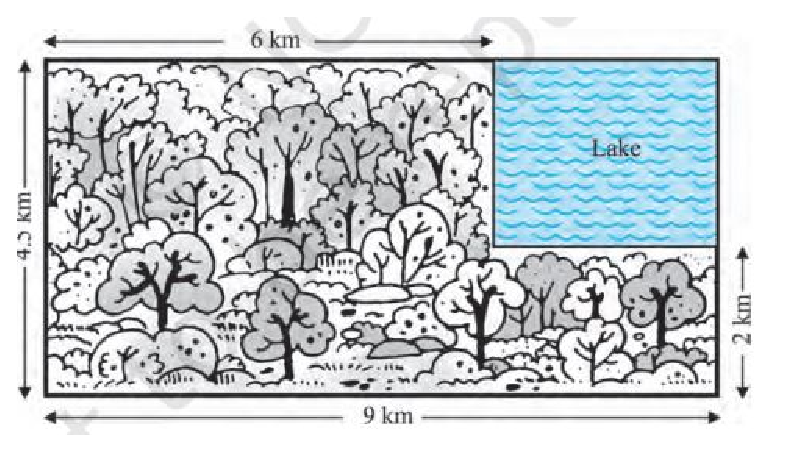
\includegraphics[width=\columnwidth]{./prob/figs/lake.eps}
\caption{}
\label{fig:lake}
\end{figure}
\solution
\begin{table}[h!]
    \label{Table-1}
    \caption{Dimensions}
    \centering
   
    \begin{tabular}{|c|c|}
    \hline
        variables & Description\\
        \hline
        l&Length of the lake\\
        \hline
        w&Width of the lake\\
        \hline
        a&Area of the lake\\
        \hline
        L&Length of the whole region\\
        \hline
        W&Width of the whole region\\
        \hline
        A&Area of the whole region\\
        \hline
    \end{tabular}
\end{table}
\begin{align}
l &= (9-6)kms\\
  &= 3kms 
\end{align}
\begin{align}
w&=(4.5-2)kms\\
 &=2.5kms
\end{align}
As the lake is rectangular;
\begin{align}
a &={l}\times{w}\\
&={3kms}\times{2.5kms}\\
&=7.5sq.kms
\end{align}
$$L=9kms$$
$$W=4.5kms$$
The whole region is of rectangular shape. Hence the area of the whole region is;
\begin{align}
A &={L}\times{W}\\
&={9kms}\times{4.5kms}\\
&=40.5sq.kms
\end{align}
\begin{table}[h!]
    \label{Table-2}
    \caption{Events and Probabilities}
    \centering
    \begin{tabular}{|c|c|}
    \hline
        variables & Description\\
        \hline
        X&Helicopter getting crashed inside lake\\
        \hline
        Y&Helicopter getting crashed outside lake\\
        \hline
        P(X)&Probability of occurrence of X\\
        \hline
        P(Y)&Probability of occurrence of Y\\
        \hline
    \end{tabular}
\end{table}
\begin{align}
    P(X)&=\frac{a}{A}\\
    &=\frac{7.5sq.kms}{40.5sq.kms}\\
    &=\frac{5}{27}=0.185
\end{align}

   \item On one page of a telephone directory, there were 200 telephone numbers.
The frequency distribution of their unit place digit (for example, in the number 25828573, the unit place digit is 3) is given in Table \ref{table:prob_exam4}
below

\begin{table}[!ht]
\centering
\resizebox{\columnwidth}{!}{
\begin{tabular}{ |c|c|c|c|c|c|c|c|c|c|c| } 
\hline
 \textbf{Digit} &0 &1 &2 &3 &4 &5 &6 &7 &8 &9 \\ 
 \hline
 \textbf{Frequency} &22 &26 &22 &22 &20 &10 &14 &28 &16 &20 \\ 
 \hline
\end{tabular}
}
\caption{}
\label{table:prob_exam4}
\end{table}
Without looking at the page, the pencil is placed on one of these numbers, i.e., the number is chosen at random. What is the probability that the digit in its unit place is 6?\\
\solution
Let X be the random variable representing the number of defective eggs from the ten eggs picked. X follows a  binomial distribution.  Since the probability of an egg being defective is 10\%, substituting n=10, p= 0.1 and k=0 in equation \eqref{eq:exam41_1}, 
probability that there is atleast one defective egg is 
\begin{align}
\pr{X \geq 1}&= 1 - \pr{X=0}  = 1-\brak{0.9}^{10}
\\
&=0.6513215599
\end{align}
The python code for the above problem is,
\begin{lstlisting}
.solutions/20-10/prob/codes/exam42.py
\end{lstlisting}


\item Suppose we throw a die once. (i) What is the probability of getting a number greater than 4 ? (ii) What is the probability of getting a number less than or
equal to 4 ?
\\
\solution
Let X be the random variable representing the number of defective eggs from the ten eggs picked. X follows a  binomial distribution.  Since the probability of an egg being defective is 10\%, substituting n=10, p= 0.1 and k=0 in equation \eqref{eq:exam41_1}, 
probability that there is atleast one defective egg is 
\begin{align}
\pr{X \geq 1}&= 1 - \pr{X=0}  = 1-\brak{0.9}^{10}
\\
&=0.6513215599
\end{align}
The python code for the above problem is,
\begin{lstlisting}
.solutions/20-10/prob/codes/exam42.py
\end{lstlisting}

\item  Given that the two numbers appearing on throwing two dice are different. Find the probability of the event `the sum of numbers on the dice is 4'.\\
\solution

	 Given the production yield per hectare of wheat of 100 farms of a village. 
		The following python code generates the required ogive.
	\begin{lstlisting}
	./solutions/20-30/codes/statistics/exercises/q25.py
	\end{lstlisting}


	
	\begin{figure}[!ht]
	\centering
	\includegraphics[width=\columnwidth]{./solutions/20-30/figs/statistics/exercises/ex_q25.eps}
	\caption{}
	\label{fig:q25_ogive}	
	\end{figure}
	
	\begin{table}[ht]
	%\begin{center}
    	%%%%%%%%%%%%%%%%%%%%%%%%%%%%%%%%%%%%%%%%%%%%%%%%%%%%%%%%%%%%%%%%%%%%%%
%%                                                                  %%
%%  This is the header of a LaTeX2e file exported from Gnumeric.    %%
%%                                                                  %%
%%  This file can be compiled as it stands or included in another   %%
%%  LaTeX document. The table is based on the longtable package so  %%
%%  the longtable options (headers, footers...) can be set in the   %%
%%  preamble section below (see PRAMBLE).                           %%
%%                                                                  %%
%%  To include the file in another, the following two lines must be %%
%%  in the including file:                                          %%
%%        \def\inputGnumericTable{}                                 %%
%%  at the beginning of the file and:                               %%
%%        \input{name-of-this-file.tex}                             %%
%%  where the table is to be placed. Note also that the including   %%
%%  file must use the following packages for the table to be        %%
%%  rendered correctly:                                             %%
%%    \usepackage[latin1]{inputenc}                                 %%
%%    \usepackage{color}                                            %%
%%    \usepackage{array}                                            %%
%%    \usepackage{longtable}                                        %%
%%    \usepackage{calc}                                             %%
%%    \usepackage{multirow}                                         %%
%%    \usepackage{hhline}                                           %%
%%    \usepackage{ifthen}                                           %%
%%  optionally (for landscape tables embedded in another document): %%
%%    \usepackage{lscape}                                           %%
%%                                                                  %%
%%%%%%%%%%%%%%%%%%%%%%%%%%%%%%%%%%%%%%%%%%%%%%%%%%%%%%%%%%%%%%%%%%%%%%



%%  This section checks if we are begin input into another file or  %%
%%  the file will be compiled alone. First use a macro taken from   %%
%%  the TeXbook ex 7.7 (suggestion of Han-Wen Nienhuys).            %%
\def\ifundefined#1{\expandafter\ifx\csname#1\endcsname\relax}


%%  Check for the \def token for inputed files. If it is not        %%
%%  defined, the file will be processed as a standalone and the     %%
%%  preamble will be used.                                          %%
\ifundefined{inputGnumericTable}

%%  We must be able to close or not the document at the end.        %%
	\def\gnumericTableEnd{\end{document}}


%%%%%%%%%%%%%%%%%%%%%%%%%%%%%%%%%%%%%%%%%%%%%%%%%%%%%%%%%%%%%%%%%%%%%%
%%                                                                  %%
%%  This is the PREAMBLE. Change these values to get the right      %%
%%  paper size and other niceties.                                  %%
%%                                                                  %%
%%%%%%%%%%%%%%%%%%%%%%%%%%%%%%%%%%%%%%%%%%%%%%%%%%%%%%%%%%%%%%%%%%%%%%

	\documentclass[12pt%
			  %,landscape%
                    ]{report}
       \usepackage[latin1]{inputenc}
       \usepackage{fullpage}
       \usepackage{color}
       \usepackage{array}
       \usepackage{longtable}
       \usepackage{calc}
       \usepackage{multirow}
       \usepackage{hhline}
       \usepackage{ifthen}

	\begin{document}


%%  End of the preamble for the standalone. The next section is for %%
%%  documents which are included into other LaTeX2e files.          %%
\else

%%  We are not a stand alone document. For a regular table, we will %%
%%  have no preamble and only define the closing to mean nothing.   %%
    \def\gnumericTableEnd{}

%%  If we want landscape mode in an embedded document, comment out  %%
%%  the line above and uncomment the two below. The table will      %%
%%  begin on a new page and run in landscape mode.                  %%
%       \def\gnumericTableEnd{\end{landscape}}
%       \begin{landscape}


%%  End of the else clause for this file being \input.              %%
\fi

%%%%%%%%%%%%%%%%%%%%%%%%%%%%%%%%%%%%%%%%%%%%%%%%%%%%%%%%%%%%%%%%%%%%%%
%%                                                                  %%
%%  The rest is the gnumeric table, except for the closing          %%
%%  statement. Changes below will alter the table's appearance.     %%
%%                                                                  %%
%%%%%%%%%%%%%%%%%%%%%%%%%%%%%%%%%%%%%%%%%%%%%%%%%%%%%%%%%%%%%%%%%%%%%%

\providecommand{\gnumericmathit}[1]{#1} 
%%  Uncomment the next line if you would like your numbers to be in %%
%%  italics if they are italizised in the gnumeric table.           %%
%\renewcommand{\gnumericmathit}[1]{\mathit{#1}}
\providecommand{\gnumericPB}[1]%
{\let\gnumericTemp=\\#1\let\\=\gnumericTemp\hspace{0pt}}
 \ifundefined{gnumericTableWidthDefined}
        \newlength{\gnumericTableWidth}
        \newlength{\gnumericTableWidthComplete}
        \newlength{\gnumericMultiRowLength}
        \global\def\gnumericTableWidthDefined{}
 \fi
%% The following setting protects this code from babel shorthands.  %%
 \ifthenelse{\isundefined{\languageshorthands}}{}{\languageshorthands{english}}
%%  The default table format retains the relative column widths of  %%
%%  gnumeric. They can easily be changed to c, r or l. In that case %%
%%  you may want to comment out the next line and uncomment the one %%
%%  thereafter                                                      %%
\providecommand\gnumbox{\makebox[0pt]}
%%\providecommand\gnumbox[1][]{\makebox}

%% to adjust positions in multirow situations                       %%
\setlength{\bigstrutjot}{\jot}
\setlength{\extrarowheight}{\doublerulesep}

%%  The \setlongtables command keeps column widths the same across  %%
%%  pages. Simply comment out next line for varying column widths.  %%
\setlongtables

\setlength\gnumericTableWidth{%
	77pt+%
	53pt+%
	53pt+%
0pt}
\def\gumericNumCols{3}
\setlength\gnumericTableWidthComplete{\gnumericTableWidth+%
         \tabcolsep*\gumericNumCols*2+\arrayrulewidth*\gumericNumCols}
\ifthenelse{\lengthtest{\gnumericTableWidthComplete > \linewidth}}%
         {\def\gnumericScale{\ratio{\linewidth-%
                        \tabcolsep*\gumericNumCols*2-%
                        \arrayrulewidth*\gumericNumCols}%
{\gnumericTableWidth}}}%
{\def\gnumericScale{1}}

%%%%%%%%%%%%%%%%%%%%%%%%%%%%%%%%%%%%%%%%%%%%%%%%%%%%%%%%%%%%%%%%%%%%%%
%%                                                                  %%
%% The following are the widths of the various columns. We are      %%
%% defining them here because then they are easier to change.       %%
%% Depending on the cell formats we may use them more than once.    %%
%%                                                                  %%
%%%%%%%%%%%%%%%%%%%%%%%%%%%%%%%%%%%%%%%%%%%%%%%%%%%%%%%%%%%%%%%%%%%%%%

\ifthenelse{\isundefined{\gnumericColA}}{\newlength{\gnumericColA}}{}\settowidth{\gnumericColA}{\begin{tabular}{@{}p{77pt*\gnumericScale}@{}}x\end{tabular}}
\ifthenelse{\isundefined{\gnumericColB}}{\newlength{\gnumericColB}}{}\settowidth{\gnumericColB}{\begin{tabular}{@{}p{53pt*\gnumericScale}@{}}x\end{tabular}}
\ifthenelse{\isundefined{\gnumericColC}}{\newlength{\gnumericColC}}{}\settowidth{\gnumericColC}{\begin{tabular}{@{}p{53pt*\gnumericScale}@{}}x\end{tabular}}

\begin{tabular}[c]{%
	b{\gnumericColA}%
	b{\gnumericColB}%
	b{\gnumericColC}%
	}

%%%%%%%%%%%%%%%%%%%%%%%%%%%%%%%%%%%%%%%%%%%%%%%%%%%%%%%%%%%%%%%%%%%%%%
%%  The longtable options. (Caption, headers... see Goosens, p.124) %%
%	\caption{The Table Caption.}             \\	%
% \hline	% Across the top of the table.
%%  The rest of these options are table rows which are placed on    %%
%%  the first, last or every page. Use \multicolumn if you want.    %%

%%  Header for the first page.                                      %%
%	\multicolumn{3}{c}{The First Header} \\ \hline 
%	\multicolumn{1}{c}{colTag}	%Column 1
%	&\multicolumn{1}{c}{colTag}	%Column 2
%	&\multicolumn{1}{c}{colTag}	\\ \hline %Last column
%	\endfirsthead

%%  The running header definition.                                  %%
%	\hline
%	\multicolumn{3}{l}{\ldots\small\slshape continued} \\ \hline
%	\multicolumn{1}{c}{colTag}	%Column 1
%	&\multicolumn{1}{c}{colTag}	%Column 2
%	&\multicolumn{1}{c}{colTag}	\\ \hline %Last column
%	\endhead

%%  The running footer definition.                                  %%
%	\hline
%	\multicolumn{3}{r}{\small\slshape continued\ldots} \\
%	\endfoot

%%  The ending footer definition.                                   %%
%	\multicolumn{3}{c}{That's all folks} \\ \hline 
%	\endlastfoot
%%%%%%%%%%%%%%%%%%%%%%%%%%%%%%%%%%%%%%%%%%%%%%%%%%%%%%%%%%%%%%%%%%%%%%

\hhline{|-|-~}
	 \multicolumn{1}{|p{\gnumericColA}|}%
	{\gnumericPB{\raggedright}\gnumbox[l]{Prodn.yield}}
	&\multicolumn{1}{p{\gnumericColB}|}%
	{\gnumericPB{\raggedright}\gnumbox[l]{No.of.farms}}
	&
\\
\hhline{|--|~}
	 \multicolumn{1}{|p{\gnumericColA}|}%
	{\gnumericPB{\raggedright}\gnumbox[l]{More than 50}}
	&\multicolumn{1}{p{\gnumericColB}|}%
	{\gnumericPB{\raggedright}\gnumbox[l]{100}}
	&
\\
\hhline{|--|~}
	 \multicolumn{1}{|p{\gnumericColA}|}%
	{\gnumericPB{\raggedright}\gnumbox[l]{More than 55}}
	&\multicolumn{1}{p{\gnumericColB}|}%
	{\gnumericPB{\raggedright}\gnumbox[l]{100-2=98}}
	&
\\
\hhline{|--|~}
	 \multicolumn{1}{|p{\gnumericColA}|}%
	{\gnumericPB{\raggedright}\gnumbox[l]{More than 60}}
	&\multicolumn{1}{p{\gnumericColB}|}%
	{\gnumericPB{\raggedright}\gnumbox[l]{98-8=90}}
	&
\\
\hhline{|--|~}
	 \multicolumn{1}{|p{\gnumericColA}|}%
	{\gnumericPB{\raggedright}\gnumbox[l]{More than 65}}
	&\multicolumn{1}{p{\gnumericColB}|}%
	{\gnumericPB{\raggedright}\gnumbox[l]{90-12=78}}
	&
\\
\hhline{|--|~}
	 \multicolumn{1}{|p{\gnumericColA}|}%
	{\gnumericPB{\raggedright}\gnumbox[l]{More than 70}}
	&\multicolumn{1}{p{\gnumericColB}|}%
	{\gnumericPB{\raggedright}\gnumbox[l]{78-24=54}}
	&
\\
\hhline{|--|~}
	 \multicolumn{1}{|p{\gnumericColA}|}%
	{\gnumericPB{\raggedright}\gnumbox[l]{More than 75}}
	&\multicolumn{1}{p{\gnumericColB}|}%
	{\gnumericPB{\raggedright}\gnumbox[l]{54-38=16}}
	&
\\
\hhline{|-|-|~}
\end{tabular}

\ifthenelse{\isundefined{\languageshorthands}}{}{\languageshorthands{\languagename}}
\gnumericTableEnd

	\caption{production yield using more than cumulative frequency}
	\label{table:stat_ex_q25anstable4}
	%\end{center}
	\end{table}




\item A game of chance consists of spinning an arrow which comes to rest pointing at one of the numbers 1, 2, 3, 4, 5, 6, 7, 8 (see Fig. \ref{fig:122} ), and these are equally likely outcomes. What is the probability that it will point at\\
(i) 8 ?\\
(ii) an odd number?\\
(iii) a number greater than 2?\\
(iv) a number less than 9?\\
\begin{figure}[!ht]
\centering

\includegraphics[width=\columnwidth]{./prob/figs/clock.eps}
\caption{}
\label{fig:122}
\end{figure}
\\
\solution
Let X be the random variable representing the number of defective eggs from the ten eggs picked. X follows a  binomial distribution.  Since the probability of an egg being defective is 10\%, substituting n=10, p= 0.1 and k=0 in equation \eqref{eq:exam41_1}, 
probability that there is atleast one defective egg is 
\begin{align}
\pr{X \geq 1}&= 1 - \pr{X=0}  = 1-\brak{0.9}^{10}
\\
&=0.6513215599
\end{align}
The python code for the above problem is,
\begin{lstlisting}
.solutions/20-10/prob/codes/exam42.py
\end{lstlisting}


\item Find the variance of the number obtained on a throw of an unbiased die.
\solution
%Let $X \in \{1,2,3,4,5,6\}$, be the random variable representing outcome of the die.The probability mass function(pmf) can be expressed as
\begin{align}
p_X\brak{n} = P\brak{X=n} =  \begin{cases}
			\frac{1}{6}, & \text{if $1 \leq n\leq 6$}\\
            0, & \text{otherwise}
		 \end{cases} 
\end{align}



		              
The variance (Var(X)) of this distribution can be found by definition,\\
\begin{align}
Var\brak{X} = E\brak{X^{2}}-\brak{E\brak{X}}^{2} \label{Eq:5.30:1}
\end{align}
where,
\begin{align}
E\brak{X}=\sum_{k=1}^{k=6} kp_X\brak{k}  \\
E\brak{X}=\frac{1}{6}\sum_{k=1}^{k=6} k \label{Eq:5.30:2}
\end{align}
We know that, sum of natural numbers from 1 to n is,
\begin{align}
\sum_{k=1}^{k=n} k = \frac{n\brak{n+1}}{2} \label{Eq:5.30:3}
\end{align}
By substituting the formula from \eqref{Eq:5.30:3} in \eqref{Eq:5.30:2} and n=6, We get,
\begin{align}
E\brak{X}=\frac{1}{6} \times \frac{6\times7}{2}  \\
E\brak{X}=\frac{7}{2} \label{Eq:5.30:4}
\end{align}
And,
\begin{align}
E\brak{X^{2}}=\sum_{k=1}^{k=6} k^{2}p_X\brak{k}  \\
E\brak{X^{2}}=\frac{1}{6}\sum_{k=1}^{k=6} k^{2} \label{Eq:5.30:5}
\end{align}
We know that, sum of squares of natural numbers from 1 to n is,
\begin{align}
\sum_{k=1}^{k=n} k^{2} = \frac{n\brak{n+1}\brak{2n+1}}{6} \label{Eq:5.30:6}
\end{align}
By substituting the formula from \eqref{Eq:5.30:6} in \eqref{Eq:5.30:5} and n=6, We get,
\begin{align}
E\brak{X^{2}}=\frac{1}{6} \times \frac{6\times7\times13}{6}  \\
E\brak{X^{2}}=\frac{91}{6} \label{Eq:5.30:7}
\end{align}
By substituting the values from \eqref{Eq:5.30:7} and \eqref{Eq:5.30:4} in \eqref{Eq:5.30:1}
\begin{align}
Var\brak{X} = E\brak{X^{2}}-\brak{E(X)}^{2}  \\
Var\brak{X} = \frac{91}{6} - \frac{49}{4}  \\
Var\brak{X} = \frac{70}{12}  \\
Var\brak{X} = 2.9167 \label{Eq:5.30:8}
\end{align}
\end{enumerate}


